% Chapter 5

\chapter{Intermediate version} % Main chapter title

\label{Chapter5} % For referencing the chapter elsewhere, use \ref{Chapter1} 

In this chapter the features of the intermediate version are exposed.

\section{Functional requirements}

The intermediate version (from now "gAn Web v2") is more complex than the first one. It was born from the tips and the observation of the pilot users. In this version we start to think more deeply about what functionalities are more important. The aesthetic is still not very considered at this stage (it will become important in the next stage). 
All the new required characteristics are listed in the following:

\begin{enumerate}

% 1
\item The user can insert multiple runs: separated by a semicolon (but in case of errors the system can automatically correct them replacing symbols like "-" or "," or "." with semicolons and giving a more robust service). These runs can be inserted by an input field of by a range select button: this button opens a "modal" that allows the user to choose the first run and the last, and automatically insert the comprised runs (for example, if the user inserts 30000 and 30010 the system inserts automatically all the run numbers between 30000 and 30010). This modal has a validation system, that ensures the correctness of the inserted values. It is not perfectly clear if this solution fits the needs of the users, but the tests with the whole users group will probably solve this doubt. 

% 2
\item The user can choose which kind of analysis execute. At this point there are different analysis in different versions of gAn, that an heterogeneous group of programmers are developing simultaneously and uploading on Gitlab. Gitlab is a web-based Git repository manager with tracking features based on Git. Git is a version control system (VCS) for tracking changes in computer files and coordinating work on those files among multiple people. It is primarily used for software development but it can be also used to keep track of changes in any files (definitions taken from Wikipedia, https://en.wikipedia.org/wiki/Git, https://en.wikipedia.org/wiki/GitLab). The different existing branches of the program propose different analyses, and it this stage is not clear which analyses there will be in the final version. In fact in gAn Web v2 five complete analyses exist, but in the future they may become more. They are externally very similar, but they give a different output (different output but in the same format: text and images). There is a more detailed overview of the structure of gAn in chapter 2, section 2. 
In this version is not clear if all the different analyses will be used for the final application. 

% 3
\item The configuration file is not only in text format, but also can be in XML format (it depends on the selected version of gAn). The XML ensures a stronger structure, and must be transparent to the user (he doesn't see differences between the configurator that works with a txt file and the one that works with XML). At this stage both text format and XML format are acceptable, to ensure the retro-compatibility of some analysis, but it is possible that in further versions the XML-based design will become dominant. 

%4
\item The user can choose what version of Root he wants to use for the program. Theoretically different versions of Root are perfectly compatible but it seems to be a good idea to allow the user to choose freely among the installed versions on the server.  

%5
\item The user can save images on his hard disk: he can choose from the shown images which to download by clicking on a specific download button near the image. Furthermore there is another button "Download All" with whom the user can simple download all the output images.

%6 
\item The user can download a reduced version of the root file with information about the images and the results: gAn produces this kind of files as "half-processed" during the computing, and it is not a problem to save this on the hard disk of the server in a specified folder. This file can be useful for an expert user (this root file contains more information than the application's output), so the user must have the opportunity to download this.     

% 7
\item The super-users prefer the dropdown menu than the radio button, so all the radio buttons in the program are replaced by dropdown menus.

% 8
\item The user has to access not only a png image, but also a root-image. This kind of image is interactive: the user can left-click and drag the mouse to select parts of the image and zoom them, and with a right click perform dynamically some kind of image processing (set colors, choose what kind of chart to see, modify the chart legend, translate in a 3D space the image etc). In this way each user can choose freely which information he wants to see in the image (to guarantee to the user the freedom of accessing the image).
All of this must be done by the user through a browser window. This requisite seems to be quite complex, but Root provides libraries (these libraries work well but they are poorly documented) to interact with Javascript.

% 9
\item In the homepage the user can see the run number of the last root file produced by the machine, and its creation date and time (so, he can understand what is the maximum of the range of the acceptable numbers). Also, the run number is an unit of measurement of the time, so through this number the user can have information about the progress of the experiment. This is an important point because actually in most cases users work with the last existing run or the one immediately before, but the way in which this application can help the user in the selection of the run needs to be deeply analyzed with a test with the users. 

% 10
\item There is a login system: the user must insert a password to use the system. The authentication is based on the comparison between the hash function of the inserted password and the hash function of the AEgIS password. If the password is correct the user receives a cookie, before each action in the site the server requests and checks this cookie to be sure about the identity of the user.  

\end{enumerate}

In the intermediate version there is another functional requirement. Ideally the user should have been able to select a gAn version also if not installed in the server machine: in this case the system should have been capable to automatically search on the AEgIS Gitlab repository the correct version (if existing), download it, unpack it in the server, and use it to execute the program. 
After some discussion this requirement has been deleted, because it was considered complex, basically useless, and potentially harmful (on the branches of the repository there are untested and incomplete versions, that can create if executed wrong outputs, so wrong scientific results). Manually installing the stable versions of gAn on the server seems to be a more smart way to work at this stage.


\subsection{Ambiguities (and related solutions)}

At least a point seems to be still ambiguous.
The textual output of gAn needs to be formatted in some way to be more organized and clear? 
The answer is difficult: for a non-physicists this output seems to be disordered, too long, with too many groups of information, and very difficult to understand, but on this question the pilot users (that are physicists) questioned answered that the output is clear and doesn't need to be modified or improved in any way. The only requests of the users were about the font and the font-size. To check this fact the best solution probably is to observe the behavior of the users at work, and eventually ask them information about that.
Anyway, in the second version, in case of multiple run selection, there is a "navbar" that allows the user to show only a run-result per time.


\section{Scenario-based functional analysis}

In the following there is a list of scenarios able to describe samples of interaction. In this situation the interaction is more complex than before.

\begin{enumerate}

\item The user wants to analyse the runs between 30000 and 30010, plus the run 31456, to make a comparison, he is interested both in the text-output and in the images: 
the user goes to the homepage, he is redirected to the authentication page and he does the login. If the login is successful the user returns automatically in the homepage, and he can insert the runs between 30000 and 30010 manually separating them with a semicolon or better clicking the "add range of runs" button, that opens a modal, in which the user can insert the minimum and the maximum of the range, and confirm (confirmation closes the modal redirecting the user to the homepage). After the user can add manually the run 31456 separating it from the others with a semicolon. If the inserted run numbers doesn't make sense the system shows on the page an error message. If the inserted run numbers are valid, the user can click the "send" button (before the button was red and disabled, now it is green and clickable) and start gAn. A progress bar is shown, a waiting message appears, and the user waits for some seconds (at this stage of development it is very hard to predict how much time gAn requests to execute). After some seconds the user is redirected in a page that shows the textual results: on the top of the page there is a navbar that shows the computed run numbers: the user uses this navbar to choose what part of the results to show in the screen. This bar is draggable, the user can freely move it. From this page the user can, through the button "show all images", access to another page dedicated to the images. In this page he can configure through dropdown menus the dimension, the layout, the group of the images to show (each image belongs to a group, the group depends on the detector that generates the data from that the image is generated). He can also, by clicking on a single image, access to another page, with a single image (the clicked image) that is completely accessible: the user can rotate the image, move it in a 3D space, zoom in, zoom out, select part, do some basic digital image processing and choose the kind of chart to show.   

\item The user wants to use the version 5.34 of Root (an old but stable version) to execute gAn: 
he completes the login, in the home page there is a button name "Choose Root version", clicking on this button the user is sent to a page where, he is informed about the current version of Root, and through a dropdown menu can choose among some version of Root already installed on the server (all the acceptable Root versions are installed on the server) . If the 5.34 version is one of the installed versions he can select it and confirm, the goal is achieved. If the 5.34 version is not installed, the user cannot use this version.  

\item The user wants to select the "Rug-dev" branch of gAn:
the process is very similar to the process that allows the user to choose a Root version. The user completes the login, in the home page there is a button name "Choose gAn version", clicking on this button the user is sent to a page where, he, through a dropdown menu, he can choose among some branches of gAn available on the machine. "Rug-dev" is one of these, the user can confirm and the task is completed.

\item The user wants to make the computation using only the data taken from the detector named "Mimito": the user, after the login, in the homepage can use the button "Edit Config" to the reach a page where, through some dropdown menus, he can change the configuration file of gAn. Each of the dropdown menus is related to a detector (often they are 5-6, it depends on the branch), and the option of the dropdown are "yes" or "no": if "yes" is selected the detector's data are used in the computation, if "no" they aren't. One of the dropdown menus is named "Mimito", the user select "yes" for this detector, "no" for all the others.  

\item The user wants to download all the images related to the runs 40001 and 40002:
after the login, he can insert the runs in the homepage (it is possible both by input field and by range selector. Two ways to do the same thing: although in the next version this point will be rethought), run gAn, wait the end of the execution, click "Show all images", and from here click "download all images". All the images will be downloaded in png format.

\item The user wants to download the semi-processed root file related to the runs 31111 and 31112:
the steps are the same as the steps used to download the images, but instead of the button "Show all images", the user has to use the button "download root files".     

\end{enumerate}  


\section{Prototyping}

The intermediate version is based on the first version, but it is quite different and re-building from zero the application (re-using only some parts) is maybe the smartest solution. Some pages (and functionalities) are added, some existing pages are improved. 
Also in this case the mock-ups are interactive and really working, the developer chooses to program directly with a common web-development process HTML-javascript-PHP based, to optimize the time.

In the following all modifications are explained.

\subsection{Modified pages}
The homepage:

\begin{figure}[H]
\centering
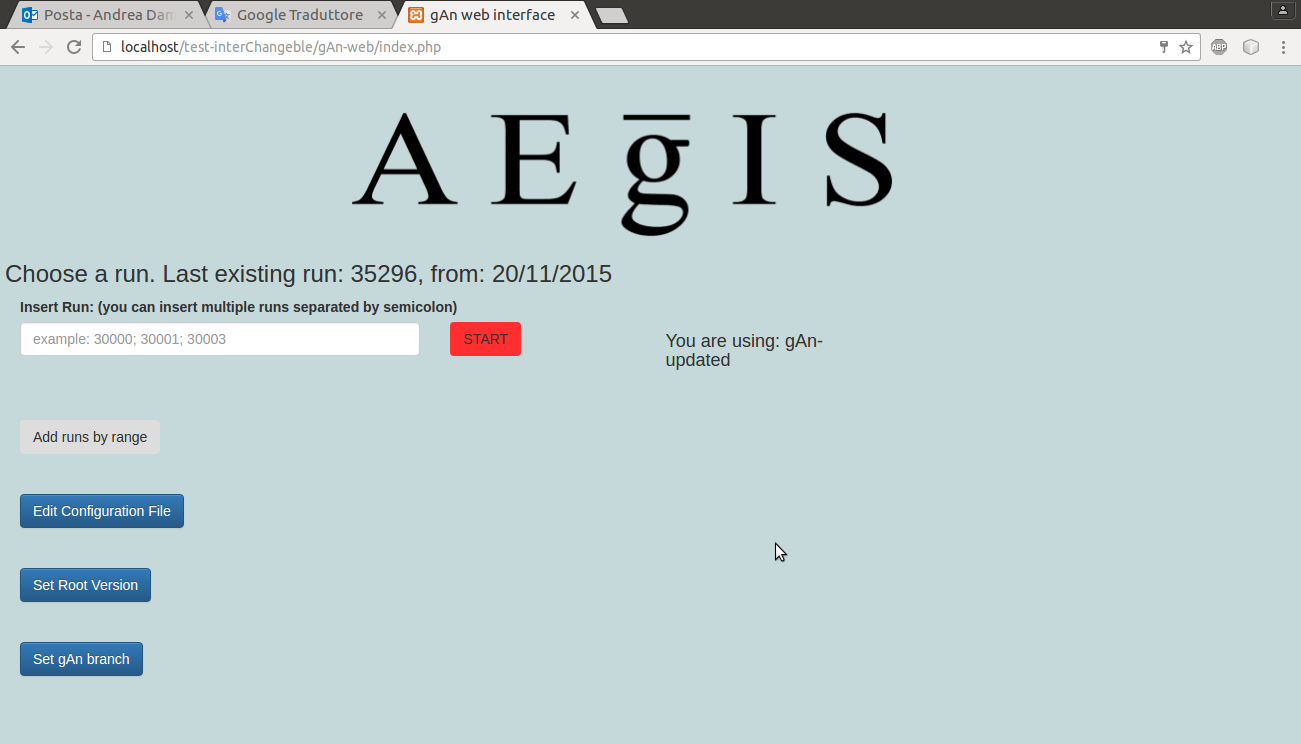
\includegraphics[scale=0.25]{HomePageEmpty.png} 
\caption{Intermediate version: the homepage of gAn Web without input}
\end{figure}


\begin{figure}[H]
\centering
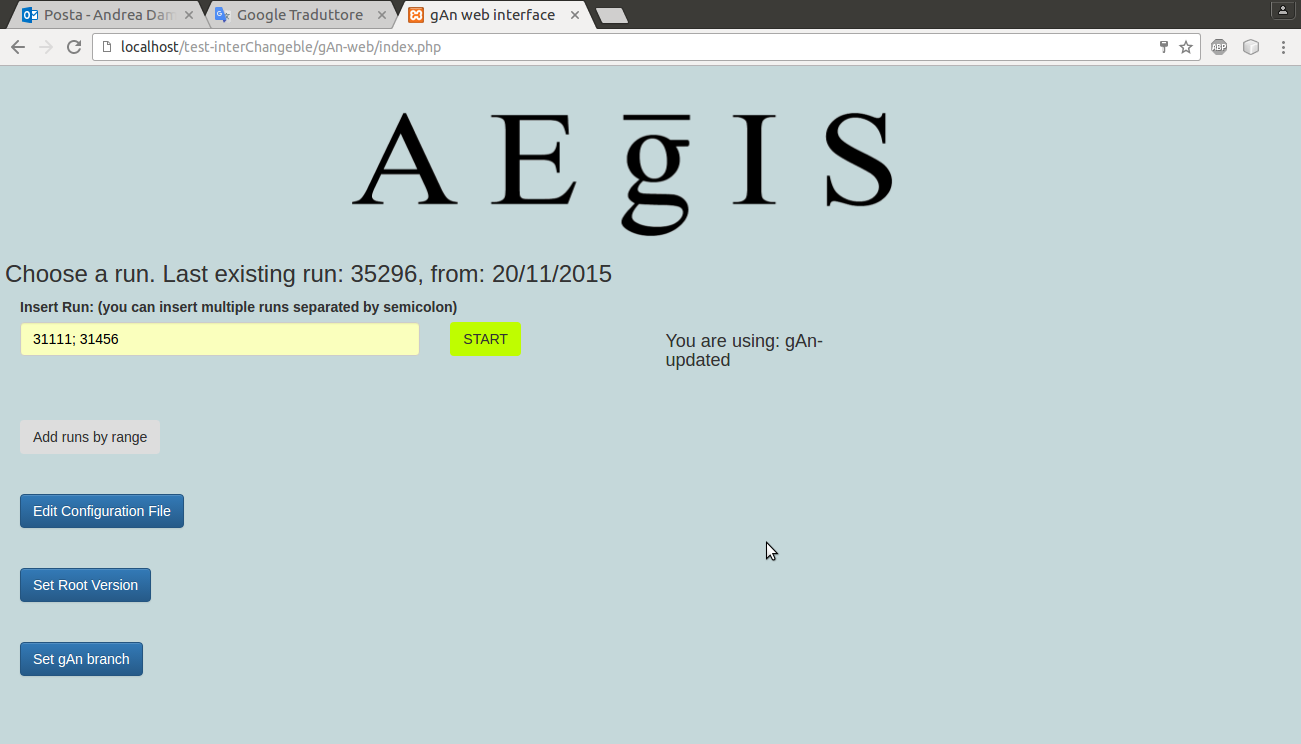
\includegraphics[scale=0.25]{HomePage.png} 
\caption{Intermediate version: the homepage of gAn Web ready to start}
\end{figure}

There are some modifications:

\begin{enumerate}

\item The user is informed about what is the last existing run: he can read "last existing run: nnnnn, from dd/mm/yy". This point is important because in most cases the user searches results regarding the lasts 2 runs.

\item The button named "send" was unclear, the word "START" is more clear, the user can immediately understand that the goal of this button is to start gAn. The button is red and disabled if there are problems (like in the following image) with the inserted runs (or if the input field is empty), green and clickable if there are no problems.	

\begin{figure}[H]
\centering
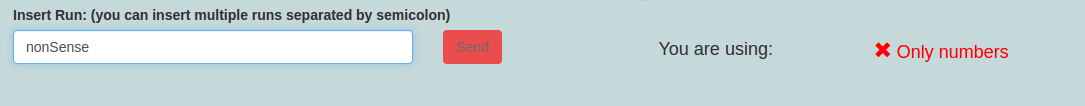
\includegraphics[scale=0.25]{ErrorInputHomepage.png}  
\caption{Intermediate version: the "Start" button is red if the values in the input field are invalid}
\end{figure}

When the user clicks start a progress bar appears. Unfortunately it is very hard to understand exactly how long the computation will last, because different runs can take different time (it depends on the amount of data that the detectors take about the run, and on the workload of the server machine, that is in common with other applications). On average has been observed that the computation takes five seconds multiplied by the number of selected runs, but there is a cache system. A wait of several seconds can be not acceptable for the user, the progress bar is imprecise but ensure to the user that the system is working correctly to ensure the correct answer. The problem is not solved: the wait time is still too long, but a solution in this case comes from the back-end, a re-factor of the code will soon make the wait time shorter. In the following image the progress bar:

\begin{figure}[H]
\centering

\includegraphics[scale=0.25]{ProgressBar.png}  
\caption{Intermediate version: the progress bar aims to make more accepttable the user's waiting}
\end{figure}



\item The input field has a place-holder, that shows to the user how to correctly insert the runs separated by semicolon (there is an automatic system that corrects the inserted values if the separator inserted by the user is not a semicolon)
 
\item It is possible to insert a group of runs selecting them by range (inserting the first and the last): the button "Add runs by range" opens a modal (shown in the image). The user can choose the minimum and the maximum value of the range, the system validates the inserted values (maximum must be more that minimum, they must be numbers etcetera).

\begin{figure}[H]
\centering
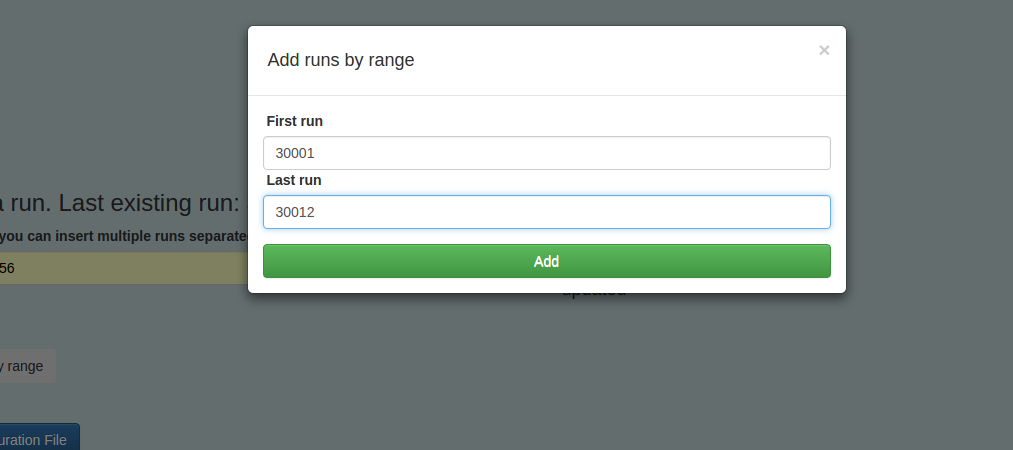
\includegraphics[scale=0.25]{RangeRunsModal.png}  
\caption{Intermediate version: the modal opened by clicking the button "Add runs by range"}
\end{figure}

\item There is a message "You are using: nameOfGAnBranch" that informs the user about which is the branch of gAn used. By default if the user doesn't change the configuration the used branch is the last used, in the last successful execution.

\item There are two new buttons: "Choose Root version", "Choose gAn version". These buttons redirect the user to pages able to modify the version of Root and gAn used in the computation.
 
\item Each button and each field have a tooltip: a text that appears when the user moves the mouse over the object. In this way an inexperienced user can easily understand what each component does.  

\end{enumerate}


The page related to the modifications of the configuration file of gAn is shown in the following:

\begin{figure}[H]
\centering
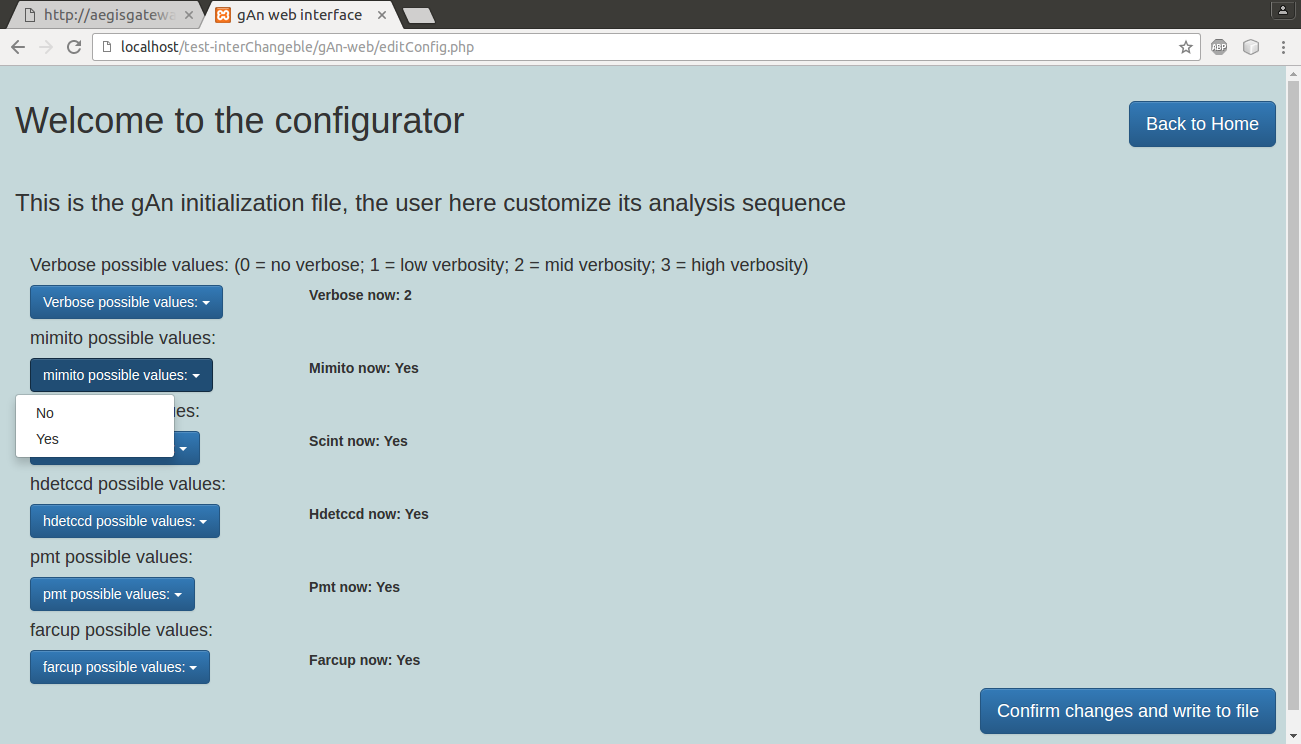
\includegraphics[scale=0.25]{EditConfig.png} 
\caption{Intermediate version: the edit-configurator page of gAn Web}
\end{figure}

This page doesn't use any more radio buttons, dropdown menus are preferred for aesthetic reasons. The user can read near the button the currently selected value for each field. 

\newpage

The page that shows the textual output of gAn is exposed in the following images, with some modifications with respect to the previous version:

\begin{figure}[H]
\centering
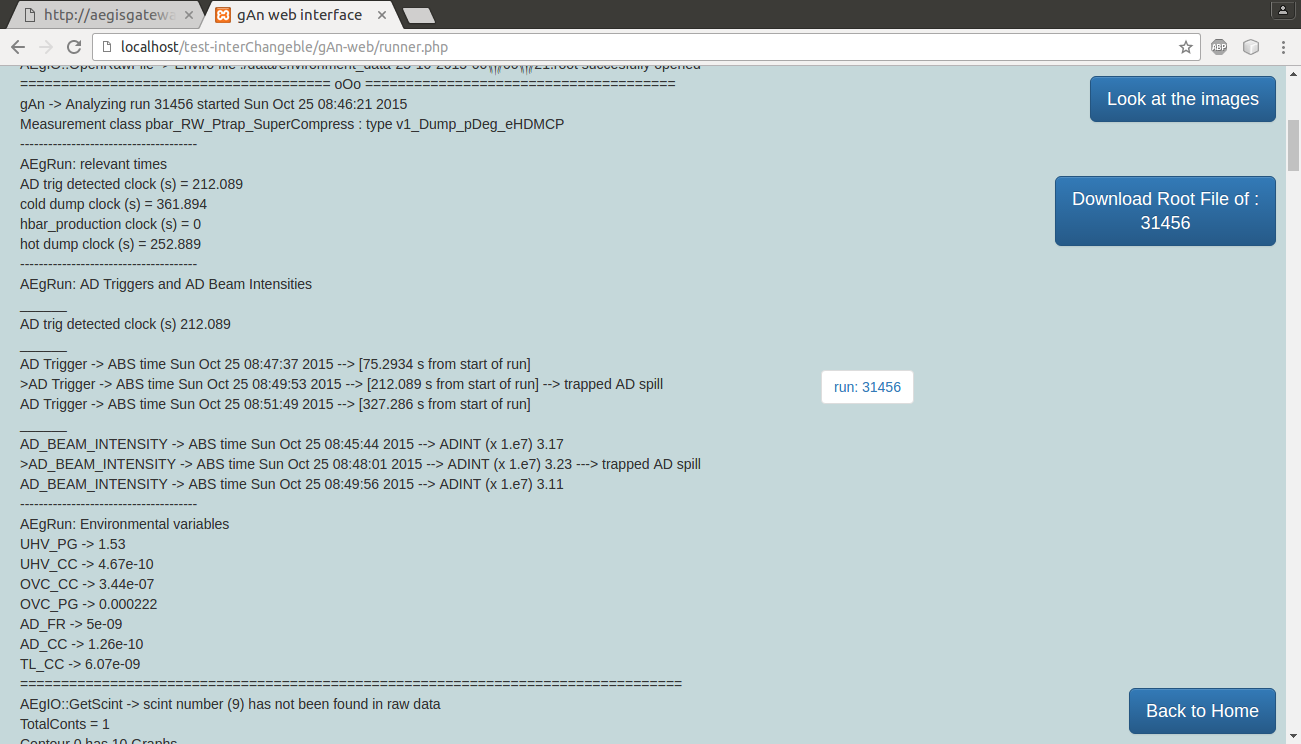
\includegraphics[scale=0.25]{TextOutputPage.png} 
\caption{Intermediate version: the page who shows the textual output of gAn}
\end{figure}


\begin{enumerate}
\item The user can choose what results he wants to show on the screen by clicking the corresponding run number from the "navbar", like in the image:

\begin{figure}[H]
\centering
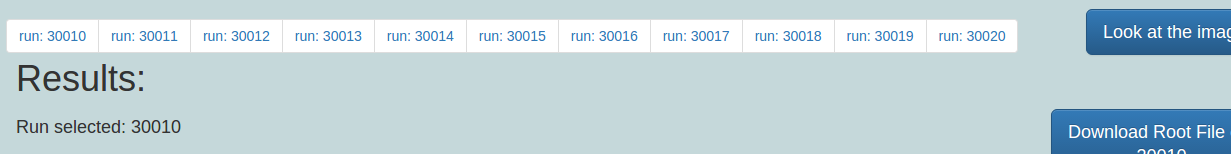
\includegraphics[scale=0.25]{WhichRunNavbar.png} 
\caption{Intermediate version: using this "navbar" the user can choose the run results to show}
\end{figure}

This navbar can be dragged by the user.

\item "Download Root File of: nnnn" is a button that allows the user to download the semi-processed file .root with some output information regarding the computation.

\item "Back to Home" gives the user the opportunity to directly return to the homepage. 

\item "Back to Home" and "Look at the images" are in a fixed position on the screen: even if the user scrolls down or up the screen he is always able to see these buttons.    

\end{enumerate}
The page that shows in an organized way the images that gAn produces in output presents a new appearance as shown in the following:



\begin{figure}[H]
\centering
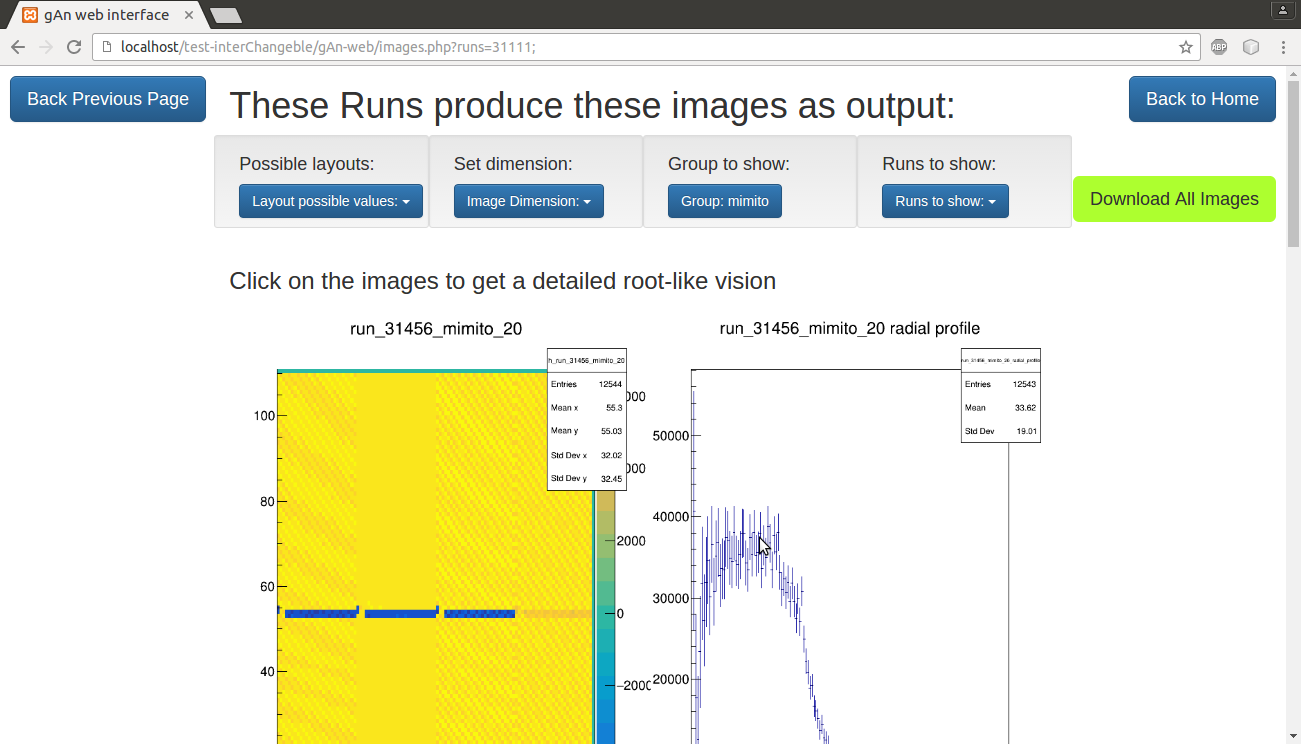
\includegraphics[scale=0.25]{AllImagesPage.png} 
\caption{Intermediate version: this page shows all the images that gAn produces in output}
\end{figure}


Modifications:
\begin{enumerate}

\item The dropdown menu "Runs to show" allows the user to select only the images produced with a single run (by default the system shows the images related to all the runs). The users widely use this option, because in this way they can compare images extrapolated in the same way but related with runs with different configurations.

\item "Download All Images" allows the user to download by a single click all the images related to the execution. The intermediate version introduces this requirement because often the users download the images using the right click of the mouse and the browser's button "Save Image As". In this way this process is faster and easier.

\item The buttons "Back to Previous page" and "Back to Home" are links towards the textual output page and the homepage. They are in fixed position.

\item By clicking on the image the user reaches a page that shows the image in full screen, but not in a static format: the image is dynamically accessible as shown in the following images:

\begin{figure}[H]
\centering
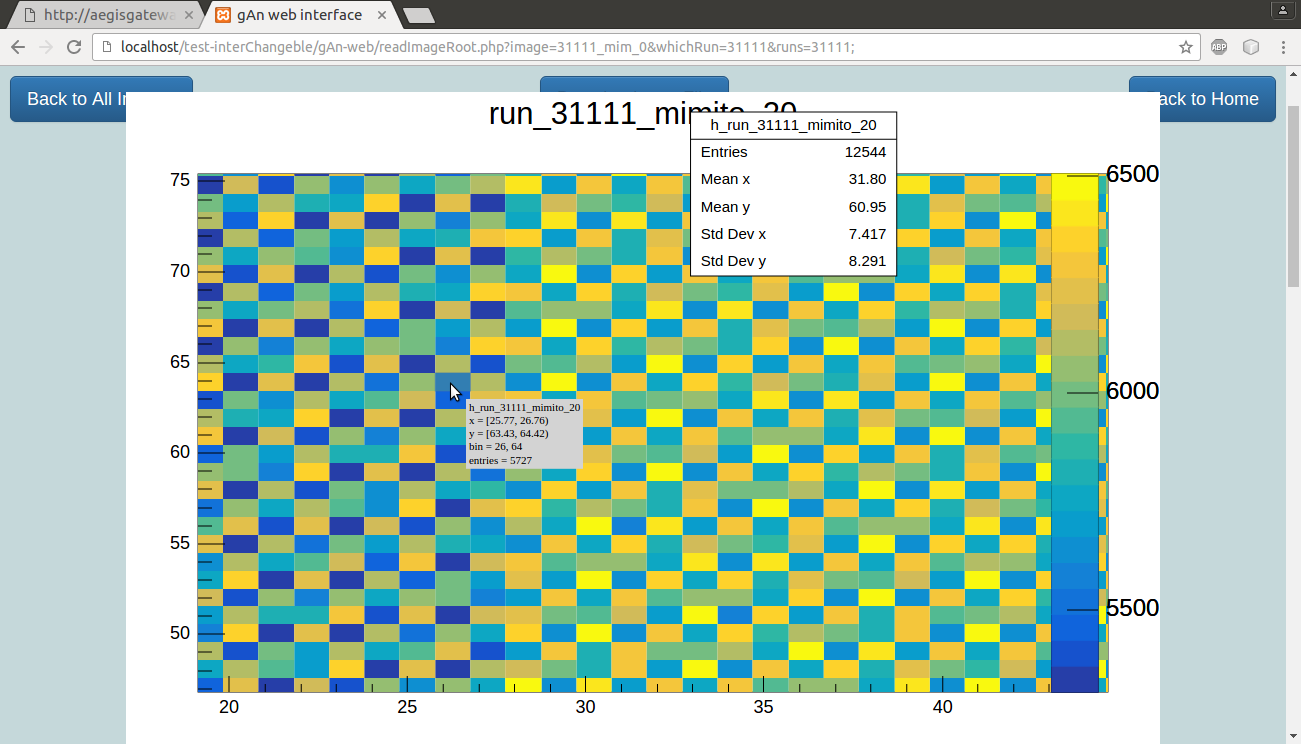
\includegraphics[scale=0.25]{RootLikeImage2.png} 
\caption{Intermediate version: moving the cursor the system shows the value of this histogram in the selected point}
\end{figure}



\begin{figure}[H]
\centering
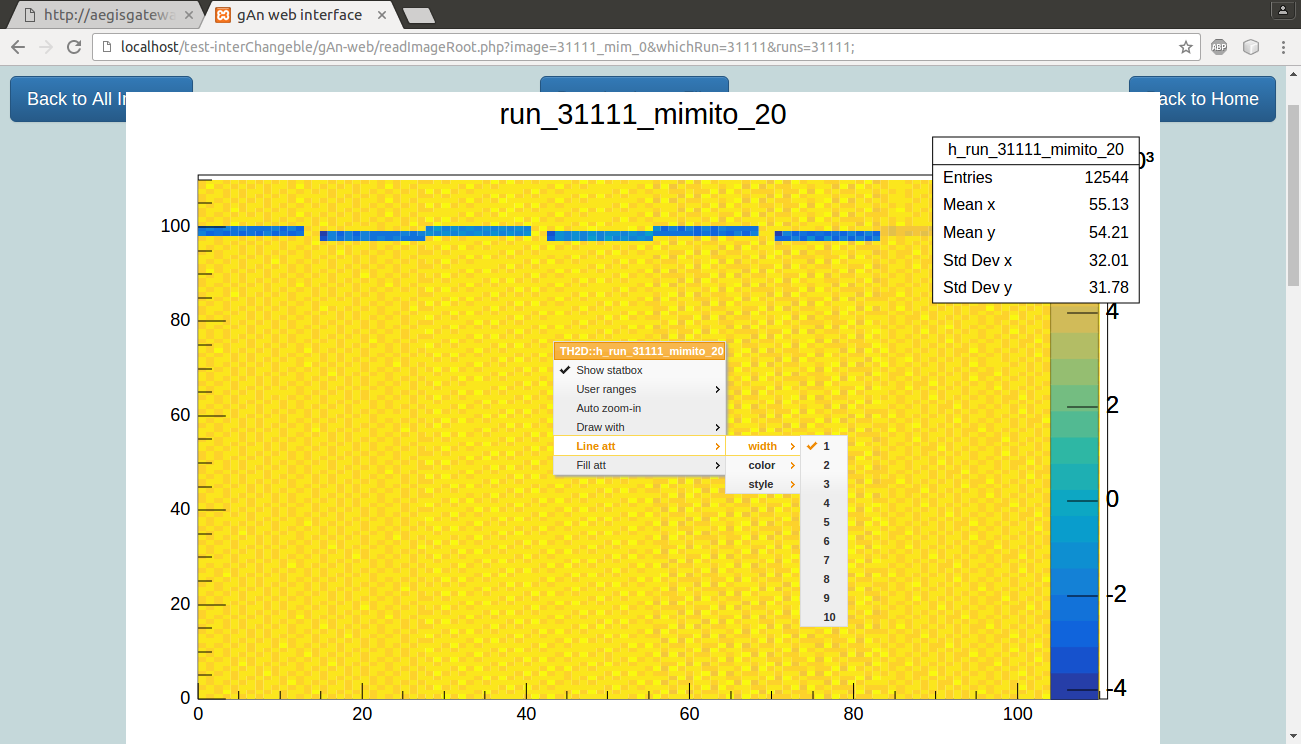
\includegraphics[scale=0.25]{RootLikeImage.png} 
\caption{Intermediate version: the user can modify numerous settings in the generated image}
\end{figure}

\begin{figure}[H]
\centering
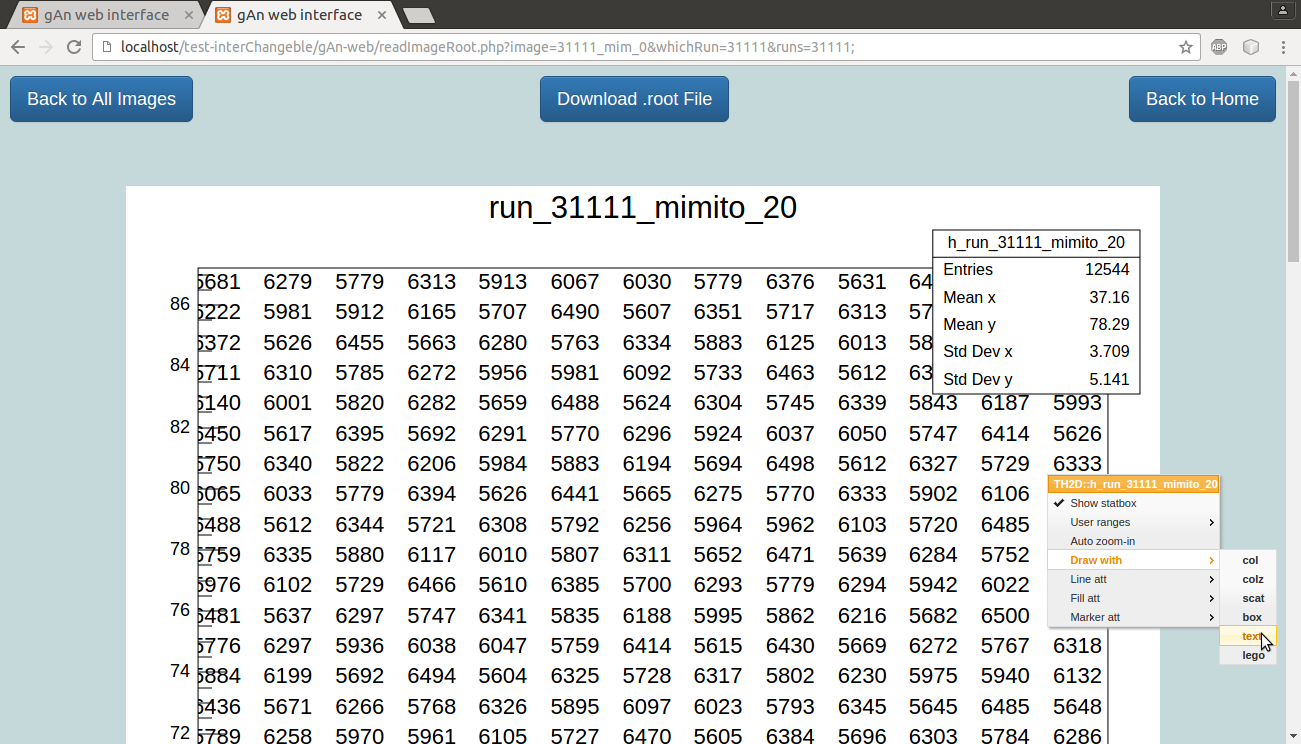
\includegraphics[scale=0.25]{RootLikeImage3.png} 
\caption{Intermediate version: the user can show the histogram not only in traditional format, but also in a numerical format where the numbers are the value of the function in their position}
\end{figure}

\begin{figure}[H]
\centering
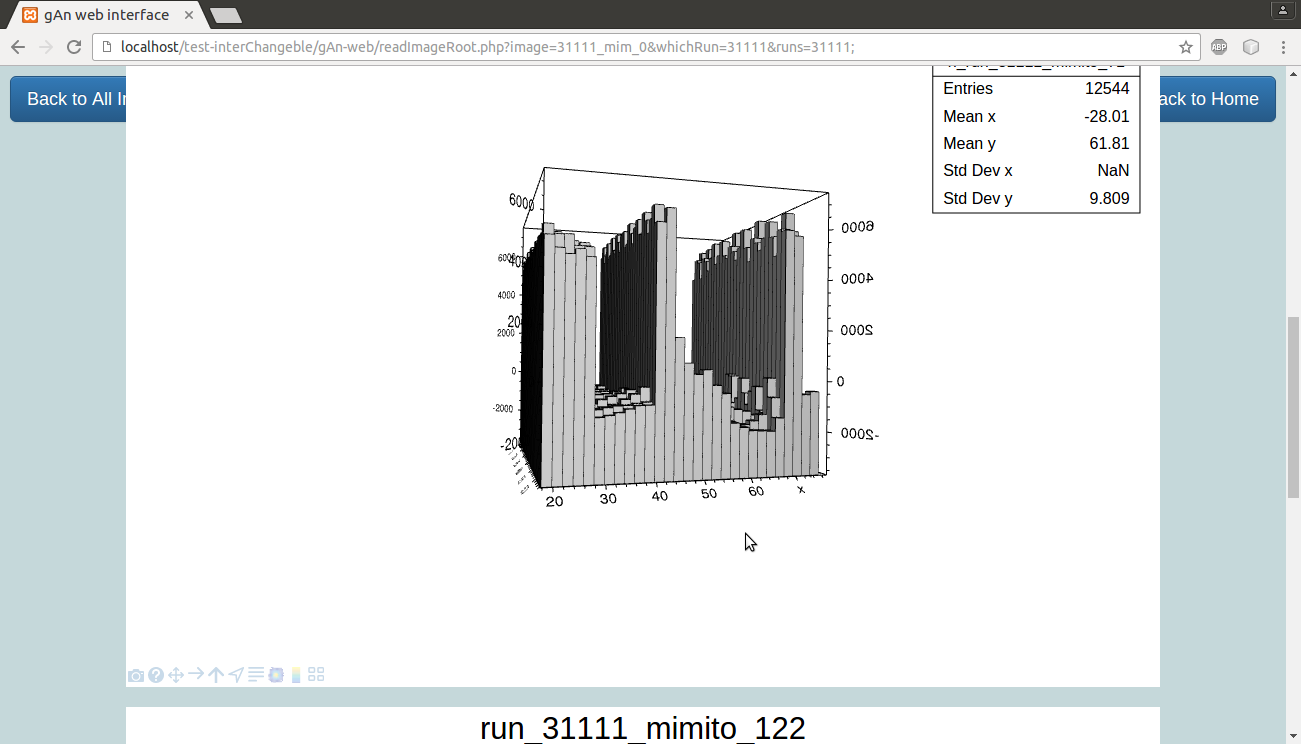
\includegraphics[scale=0.25]{RootLikeImage4.png} 
\caption{Intermediate version: another solution is to generate a 3d image in lego-style of the histogram}
\end{figure}


 
\end{enumerate}


\subsection{Added pages}

Some pages in the intermediate version are completely new, because they implement new functionalities.

The first new page that the user sees is the login page. It is very simple, it doesn't authenticate a single user, but asks only the password. This basic system of authentication aims simply to ensure that only the people that work in AEgIS experiment can use this software.

The login page image is shown in the following:

\begin{figure}[H]
\centering
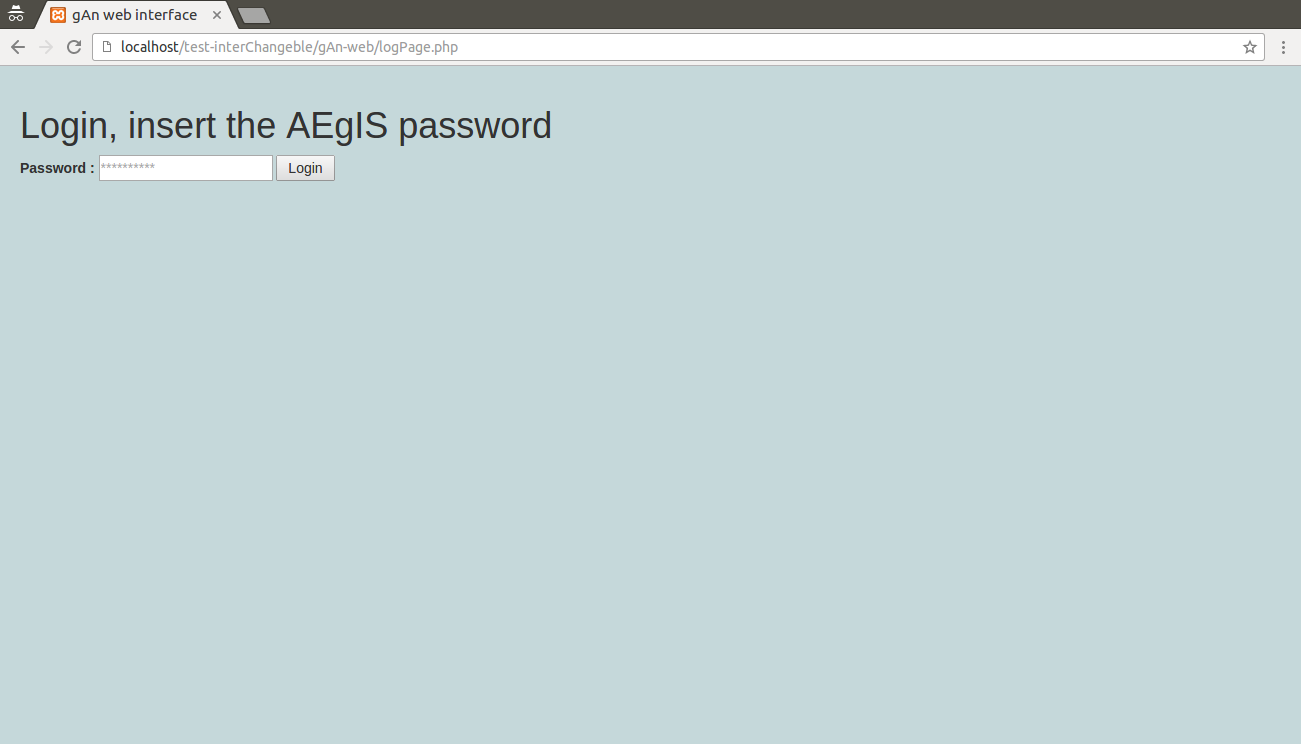
\includegraphics[scale=0.25]{Login.png} 
\caption{Intermediate version: simple login page}
\end{figure}

In this version there is also the opportunity for the user to choose which branch of gAn and which version of Root Framework can be used to execute the program. The pages that the user can visit are quite similar, and quite simple. The user must use dropdown menus to make these choices, and there is always a default safe choice (the system remembers the last working version of Root and the last working branch of gAn), so it is impossible to make errors or inconsistent choices. 

In the following there are some screen-shots of these pages

\begin{figure}[H]
\centering
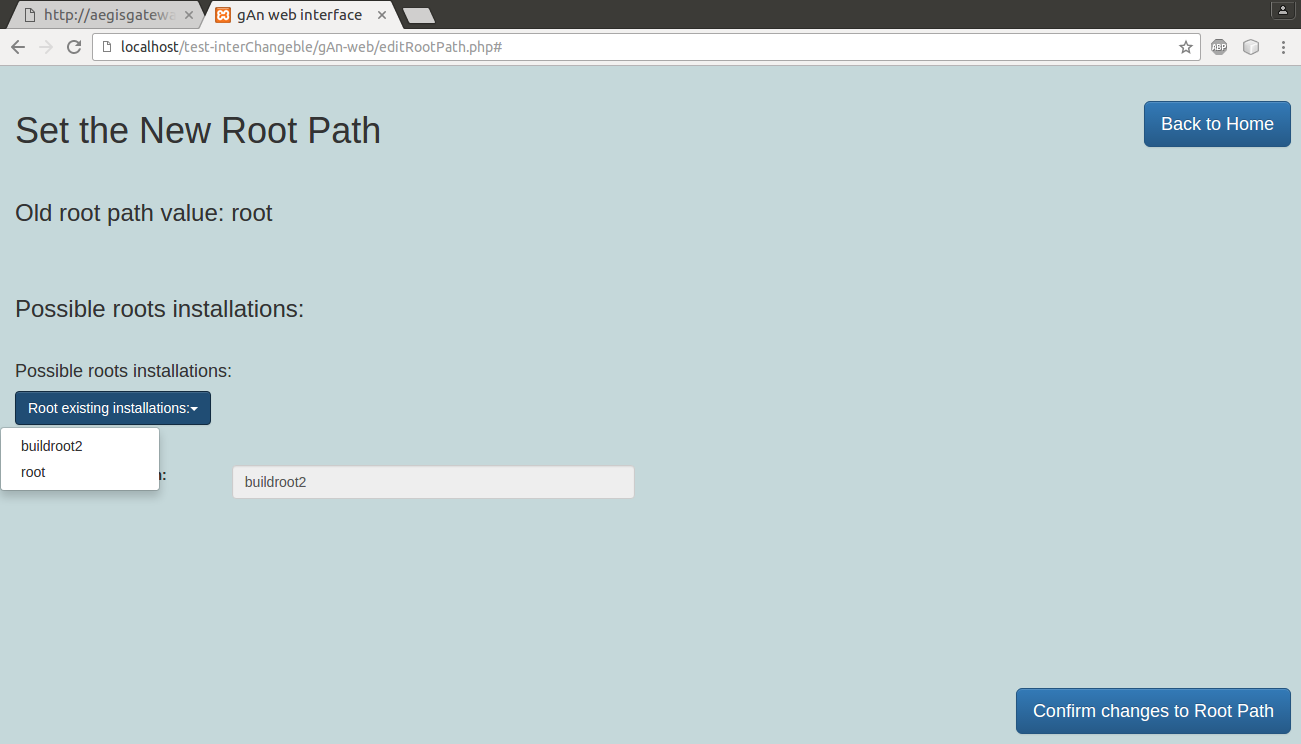
\includegraphics[scale=0.25]{RootVersionChoice.png} 
\caption{Intermediate version: page where the user can choose the Root version to use}
\end{figure}
 
 
\begin{figure}[H]
\centering
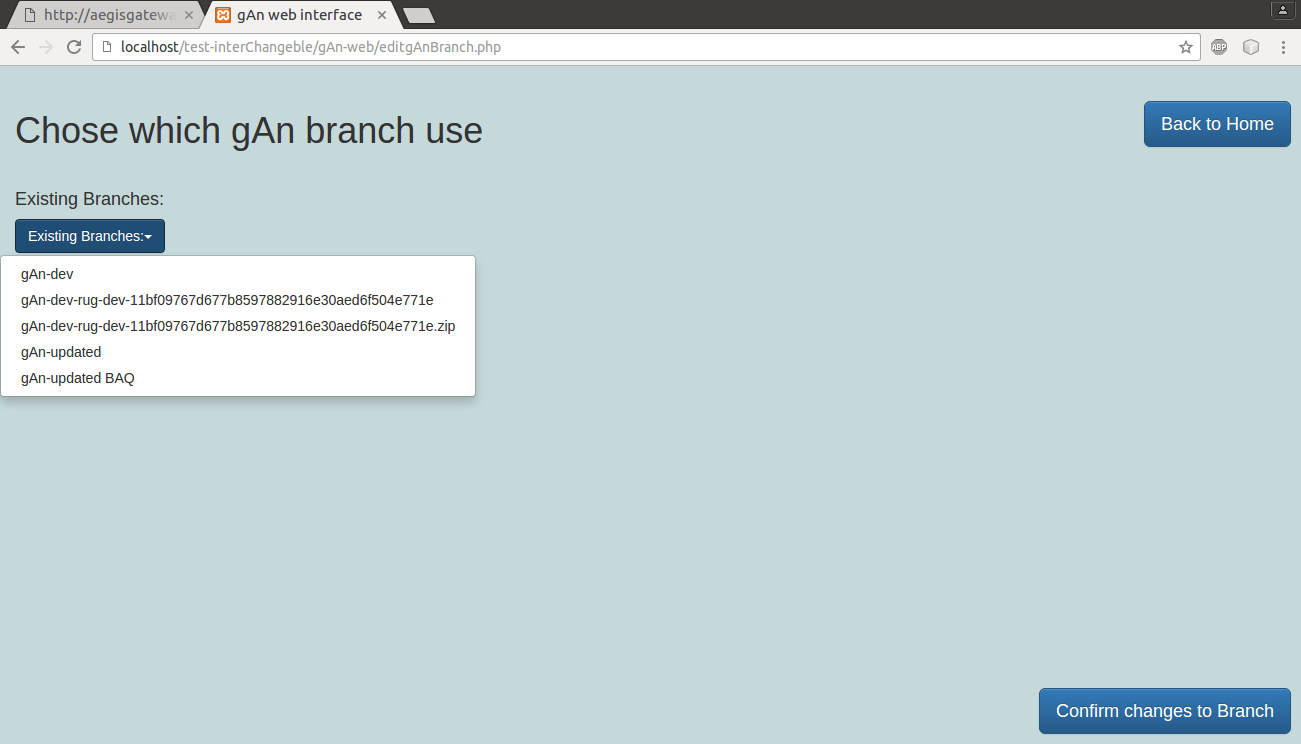
\includegraphics[scale=0.25]{ChoosegAnBranch.png} 
\caption{Intermediate version: page where the user can choose the Branch of gAn to use}
\end{figure}
